%
% dia4.tex
% 
% Copyright 2014 Rony J. Letona <rony@zronyj.com>
% 
% This program is free software; you can redistribute it and/or modify
% it under the terms of the GNU General Public License as published by
% the Free Software Foundation; either version 2 of the License, or
% any later version.
% 
% This program is distributed in the hope that it will be useful,
% but WITHOUT ANY WARRANTY; without even the implied warranty of
% MERCHANTABILITY or FITNESS FOR A PARTICULAR PURPOSE.  See the
% GNU General Public License for more details.
% 
% You should have received a copy of the GNU General Public License
% along with this program; if not, write to the Free Software
% Foundation, Inc., 51 Franklin Street, Fifth Floor, Boston,
% MA 02110-1301, USA.
%

\documentclass[10pt,letterpaper]{article}
\usepackage[latin1]{inputenc}
\usepackage[spanish]{babel}
\usepackage{graphicx}
\usepackage{hyperref}
\usepackage{amsmath}
\usepackage{amsfonts}
\usepackage{amssymb}
\usepackage{color}
\usepackage{float}
\usepackage[left=2cm,right=2cm,top=2cm,bottom=2cm]{geometry}
\usepackage{natbib}
\bibliographystyle{apa}
\author{Rony J. Letona}
\title{Taller de Qu\'imica Computacional Aplicada: D\'ia 4}
\definecolor{light-gray}{gray}{0.90}

\newcommand{\tab}[1]{\hspace{.2\textwidth}\rlap{#1}}

\newcommand{\inlinecode}[1]{
\colorbox{light-gray}{\texttt{#1}}
}

\newsavebox{\selvestebox}
\newenvironment{Code}
{
\begin{lrbox}{\selvestebox}%
\begin{minipage}{\dimexpr\columnwidth-2\fboxsep\relax}
\fontfamily{\ttdefault}\selectfont
}
{\end{minipage}\end{lrbox}%
\begin{center}
\colorbox{light-gray}{\usebox{\selvestebox}}
\end{center}
}

\newcommand{\Picture}[1]
{
	\begin{figure}[H]
	\begin{flushleft}
	\includegraphics[width=\columnwidth]{#1}
	\end{flushleft}
	\end{figure}
}

\begin{document}
\maketitle

\section{Ejercicios con \LaTeX\ }
Los reportes son una de las cosas con las que m\'as nos topamos tanto en un ambiente acad\'emico, como en uno laboral. Si no estamos tratando de explicar por qu\'e no nos sali\'o el producto en la s\'intesis, estamos buscando c\'omo ligar la evidencia de un an\'alisis y que eso nos lleve a una explicaci\'on. Adem\'as, siempre debemos documentar cada paso realizado. Sin embargo, hay una cosa que suele quitarnos m\'as de nuestro preciado tiempo: el formato. Cuando comenz\'abamos a hacer reportes en los primeros a\~nos fuimos ingenuos y los hicimos todos desde cero. Adem\'as, muchas veces nos los pidieron a hechos a mano. Luego ya no fue as\'i, pero cada instructor o catedr\'atico nos los ped\'ia diferentes. Al final de cuentas siempre result\'abamos haciendo una plantilla para ese laboratorio y la segu\'iamos usando todo el semestre. Si bien nos iba, la plantilla era buena y agregarle cosas no nos arruinaba cosas como la numeraci\'on de las p\'aginas o la colocaci\'on de las im\'agenes, pero si no, nos iba a tomar unos 20 minutos arreglar el problema. Adem\'as de esto, ni nuestros proyectos, ni nuestros reportes se vieron profesionales. Acept\'emoslo, nunca se hab\'ian visto como un art\'iculo cient\'ifico, como un peque\~no manual o como un libro. ``Eso es trabajo de una editorial.''--pensar\'ian algunos. Pero hoy vamos a ver que no, y que hacer trabajos con un acabado de editorial no es nada complicado.\\

Hace ya varios a\~nos se intent\'o crear un programa que facilitara la impresi\'on de documentos en cualquier tipo de impresora; desde impresoras de matriz hasta impresoras laser. Este programa se hizo llamar \TeX\ y su desarrollo llev\'o a que sea utilizado por editoriales grandes hasta nuestros d\'ias. El ``dialecto'' m\'as utilizado de \TeX\ hoy d\'ia es llamado \LaTeX\ . Este result\'o siendo el lenguaje de programaci\'on adoptado por la comunidad cient\'ifica en muchas partes por sus ventajas para crear plantillas, escribir ecuaciones, numerarlas, insertar bibliograf\'ias, autonumerar p\'aginas, etc. Se dice que es un lenguaje de programaci\'on como HTML, pues se basa en peque\~nas palabras indicando las diferentes partes del documento. Y la idea final es obtener un documento que no solo tenga un contenido ideal, como solemos inclu\'irselos a nuestros proyectos, sino que se vea excepcional sin tener que invertir mucho tiempo en darle formato. Pero para qu\'e explicar lo bien que se puede ver un documento de estos? Es un poco redundante. El documento que estamos viendo fue hecho en \LaTeX\ , al igual que el de ayer, anteayer y el de los dem\'as d\'ias. Pero la idea no es que lo sepamos identificar en un documento, sino que lo sepamos usar. Comencemos, pues, a crear nuestros documentos de una forma diferente!

\subsection{Comenzando con un Proyecto}
Para trabajar con \LaTeX\ suele no hacer falta nada m\'as que un editor de texto y saber c\'omo crear un archivo \emph{PDF} a partir del archivo \TeX . Sin embargo, siendo \LaTeX\ tan extenso, vamos a utilizar un editor en espec\'ifico. Con este podremos ahorrarnos muchos problemas a la hora de crear nuestros documentos. Como primer paso, vamos a abrir \textbf{\TeX Maker} y all\'i vamos crear un documento nuevo. Este nuevo archivo en blanco lo vamos a guardar como \emph{proyecto\_01.tex}. Ahora vamos a iniciar con nuestro proyecto.\\

Vamos a iniciar el documento escribiendo:
\begin{Code}
\begin{verbatim}
\documentclass[12pt,letterpaper]{article}

\begin{document}

\end{document}
\end{verbatim}
\end{Code}

Aqu\'i iniciamos especificando el tama\~no de letra que se utilizar\'a en todo el documento, y el tama\~no de p\'agina con el que se trabajar\'a. Finalmente, en la primera l\'inea vemos que se especifica que vamos a crear un art\'iculo. Hay otras opciones como \inlinecode{letter}, \inlinecode{report} y \inlinecode{book}. La diferencia entre ellos son los comandos y la forma de aplicar el formato (el libro utiliza cap\'itulos, la carta solicita encabezados, fechas y firma, el reporte es como un informe final de proyecto, etc). Luego especificamos en d\'onde deseamos tener el contenido del documento: entre el inicio y el final del documento. All\'i dentro vamos a poner el contenido del archivo \emph{lorem\_ipsu.txt} (c\'opialo y p\'egalo). Luego, en la barra superior de \textbf{\TeX Maker} vas a hallar dos flechas azul claro. A la par de la primera debe de decir PDFLaTeX y a la par de la segunda debe decir View PDF. La idea all\'i es tener configurada la parte que nos permitir\'a transformar nuestro archivo \TeX\ en un PDF y poder visualizarlo despu\'es.

\Picture{img/tex_01.png}

Cuando esas dos cosas ya est\'en como en la im\'agen, podemos presionar la primera flecha azul. En la barra de abajo deber\'ia de aparecer algo que nos diga que el proceso ha terminado exitosamente. Ahora presionaremos la segunda flecha azul y el resultado nos ser\'a revelado: un documento escrito con un estilo bastante limpio y hasta con p\'aginas numeradas. Genial! Ahora ... hay ciertas cosas que no se ven muy bien. En primer lugar, vamos a agregar espacios entre p\'arrafos. Para ello, agregaremos dos diagonales inversas \inlinecode{\textbackslash \textbackslash } al terminar de cada p\'arrafo: despu\'es del punto y volvemos a presionar ambas flechas.\\

Ahora ya separamos los p\'arrafos y nuestro documento ya se ve mejor. Antes de proceder a la siguiente secci\'on repasemos en lo que hicimos. Inicializamos un documento especificando un tama\~no de letra y de p\'agina. Luego colocamos algo de texto dentro de \'el y finalmente separamos los p\'arrafos con una diagonal doble inversa. No es tan complicado, aunque s\'i requiere un poco de tiempo. Pero lo m\'as importante: no se ve como nosotros queremos que se vea. Para ello, vamos a continuar.

\subsubsection{Geometr\'ia}

Hasta ahora, si pensamos en c\'omo se ve nuestro documento, vamos a notar que los m\'argenes son muy grandes. Generalmente esto es algo que solo cambiamos cuando deseamos que la cantidad de p\'aginas en nuestros proyectos sea mayor o menor. En este caso, sin embargo, estamos desperdiciando demasiado espacio en los m\'argenes. C\'omo corregimos eso? La forma de cambiar m\'argenes en \LaTeX\ es m\'as sencilla de lo que uno se imagina, y suele hacerse siempre al inicio de los documentos que vayamos a producir. En nuestro caso, dejaremos m\'argenes de $2cm$ mediante el uso del paquete \inlinecode{geometry}. El resultado ser\'a algo as\'i:

\begin{Code}
\begin{verbatim}
\documentclass[12pt,letterpaper]{article}
\usepackage[left=2cm,right=2cm,top=2cm,bottom=2cm]{geometry}

\begin{document}

Lorem ipsum dolor ...

\end{document}
\end{verbatim}
\end{Code}

Al volver a correr esto con las dos flechas azules, nos damos cuenta de que nuestro resultado es mucho mejor. Ya se nota que tiene un toque de documento. Y la mejor parte es que \LaTeX\ usa sangr\'ias en cada p\'arrafo y los deja justificados a\'un utilizando guiones! Se ve bastante bien.

\subsubsection{Idiomas}

Ahora agregaremos un par de paquetes m\'as que nos permitir\'an escribir lo que nosotros querramos dentro de nuestro documento. Y es que \LaTeX\ fue dise\~nado originalmente para el idioma ingl\'es. Un ejemplo de eso es que \textbf{las tildes} y \textbf{la \~n} no las podemos escribir f\'acilmente. Pero m\'as que eso, los guiones para dividir una palabra son importantes. Para ello, vamos a agregar otro paquete en el documento que llevamos.

\begin{Code}
\begin{verbatim}
\documentclass[12pt,letterpaper]{article}
\usepackage[left=2cm,right=2cm,top=2cm,bottom=2cm]{geometry}
\usepackage[spanish]{babel}

\begin{document}

Lorem ipsum dolor ...

\end{document}
\end{verbatim}
\end{Code}

Con esto ya muchas cosas se nos permiten en espa\~nol. M\'as adelante vamos a ver qu\'e impacto tiene realmente eso. Ahora, vamos a ver dos alternativas para lograr escribir las tildes y la \~n. La forma \emph{complicada} de escribirlas en \LaTeX\ es as\'i:

\begin{Code}
\begin{verbatim}
\'a
\'e
\'i
\'o
\'u
\~n
\end{verbatim}
\end{Code}

Ahora, a pesar de que parece bastante tedioso escribir de esa manera, es la \'unica infalible. Aunque el documento est\'e configurado para ingl\'es, esto garantiza que podamos tener tildes y \~ns. La otra forma de hacerlo sin complicarnos tanto la vida es incluyendo otro paquete en nuestro documento: un conjunto de caracteres universal.

\begin{Code}
\begin{verbatim}
\documentclass[12pt,letterpaper]{article}
\usepackage[left=2cm,right=2cm,top=2cm,bottom=2cm]{geometry}
\usepackage[utf8]{inputenc}
\usepackage[spanish]{babel}

\begin{document}

Lorem ipsum dolor ...

\end{document}
\end{verbatim}
\end{Code}

Con este paquete ya no necesitamos estar usando el gui\'on y las ap\'ostrofes, sino que podemos escribir libremente y no habr\'an problemas. En este caso en particular, estos documentos est\'an escritos de la primera manera para garantizar que quien no posea el paquete en su ordenador, pueda de todas formas armar estos documentos. Sin embargo, la brecha de idiomas ya la cubrimos. Ahora solo vamos a profundizar en una \'ultima cosa: paquetes.\\

\subsubsection{Paquetes}

Los paquetes son formas de extender las funciones normales de \LaTeX . Como ya hemos visto, usamos paquetes para los m\'argenes, para el conjunto de caracteres permitidos y para idioma. Existen paquetes para muchas otras cosas m\'as. La sintaxis para incluirlos, sin embargo, es siempre la misma: \inlinecode{\textbackslash usepackage\{\emph{paquete}\}}\\

Todav\'ia vamos a ver aqu\'i un paquete m\'as: encabezados y pies de p\'agina. Este nos dar\'a una idea de qu\'e hacer y c\'omo darle una forma m\'as elegante a nuestros documentos.\\

\subsubsection{Encabezado y Pie}

El encabezado y pie de p\'agina suele ser todo un rollo en Microsoft Word. Estos suelen necesitar mucha configuraci\'on y bastante paciencia. En \LaTeX\ el asunto no es tan diferente, pero veremos que existen algunas ventajas que nos facilitar\'an el proceso. Comencemos importando el paquete que nos permitir\'a hacer el encabezado y el pie.\\

\begin{Code}
\begin{verbatim}
\documentclass[12pt,letterpaper]{article}
\usepackage[left=2cm,right=2cm,top=2cm,bottom=2cm]{geometry}
\usepackage[utf8]{inputenc}
\usepackage[spanish]{babel}
\usepackage{fancyhdr}
\pagestyle{fancy}

\begin{document}

Lorem ipsum dolor ...

\end{document}
\end{verbatim}
\end{Code}

Si ponemos atenci\'on, notaremos que no solo incluimos un paquete, sino que le pedimos un estilo particular a la p\'agina. Lo que hace esto es que construye un estilo de encabezado y pies de p\'agina basados en el n\'umero de la p\'agina y en la secci\'on o cap\'itulo que se halle en esa p\'agina. Ahorita aunque re-armemos nuestro PDF no lo notaremos (solo notaremos una delgada l\'inea en el encabezado), pero en la siguiente secci\'on esto se har\'a evidente.\\

Si deseamos cambiar la manera en que est\'an ensamblados el encabezado y el pie de p\'agina, esto se puede hacer. No se cubrir\'a en este documento, puesto que es un poco largo, pero es importante mencionar que se puede hacer y no es nada complicado.

\subsection{Decorando el Documento}
\subsubsection{T\'itulo}
Ahora que ya tenemos un formato general para nuestro documento, lo vamos a comenzar a decorar un poco. Lo primero que vamos a agregarle ser\'a un t\'itulo. Pero para eso necesitamos especificar 2 cosas: el autor y el t\'itulo de nuestro trabajo. En este caso, el autor vamos a ser nosotros mismos y el t\'itulo ser\'a: Lorem Ipsum. El c\'odigo se ver\'a ahora algo as\'i:

\begin{Code}
\begin{verbatim}
\documentclass[12pt,letterpaper]{article}
\usepackage[left=2cm,right=2cm,top=2cm,bottom=2cm]{geometry}
\usepackage[utf8]{inputenc}
\usepackage[spanish]{babel}
\usepackage{fancyhdr}
\pagestyle{fancy}
\author{Mi Nombre}
\title{Lorem Ipsum}

\begin{document}

\maketitle

Lorem ipsum dolor ...

\end{document}
\end{verbatim}
\end{Code}

Notemos que dentro del documento incluimos una peque\~na palabra nueva: \inlinecode{\textbackslash maketitle} Es justo aqu\'i que el t\'itulo es incluido dentro de nuestro documento. Si no lo incluimos, ninguna de las otras 2 entradas tienen sentido. El resultado al armar nuestro documento en PDF es algo vistoso, pero cumple con lo que dese\'abamos. Adem\'as, incluye la fecha actual en espa\~nol (otra cosa que sale de usar el paquete para espa\~nol). Es importante darnos cuenta de que al incluir el t\'itulo, el encabezado ya no apareci\'o en esa p\'agina! Y hablando de encabezados, vamos a pasar a otra cosa que nos sirve de mucho al elaborar un documento nuevo.

\subsubsection{Secciones y Cap\'itulos}
Dividir un documento en diferentes partes suele hacerlo m\'as f\'acil de leer adem\'as de hacerlo m\'as f\'acil de referenciar. \LaTeX\ suele requerir que nosotros indiquemos d\'onde hay cap\'itulos y/o secciones para poder as\'i armar \'indices o sacar referencias. Antes de comenzar vamos a aclarar algo: Las secciones pueden ser utilizadas en cualquier documento. Los cap\'itulos solo pueden ser usados en reportes o libros.\\

En este caso estamos trabajando con un art\'iculo, as\'i que vamos a agregarle diferentes secciones a nuestro documento. Pero para que se note la diferencia, vamos a agregar m\'as texto. Vamos a abrir todos los documentos \emph{ipsum} en nuestro directorio y los vamos a agregar con sus respectivos nombres como secciones (recuerda separar los p\'arrafos):

\begin{Code}
\begin{verbatim}
\documentclass[12pt,letterpaper]{article}
\usepackage[left=2cm,right=2cm,top=2cm,bottom=2cm]{geometry}
\usepackage[utf8]{inputenc}
\usepackage[spanish]{babel}
\usepackage{fancyhdr}
\pagestyle{fancy}
\author{Mi Nombre}
\title{Lorem Ipsum}

\begin{document}

\maketitle

\section{Lorem Ipsum}
Lorem ipsum dolor sit amet ...

\section{Bacon Ipsum}
Bacon ipsum dolor sit amet corned beef ...

\section{Cupcacke Ipsum}
Cupcake ipsum dolor sit amet candy canes ...

\section{Hipster Ipsum}
Before they sold out swag Pitchfork roof ...

\section{Tuna Ipsum}
Squaretail; ghost flathead hatchetfish ...

\section{Veggie Ipsum}
Veggies es bonus vobis, proinde vos postulo ...

\end{document}
\end{verbatim}
\end{Code}

Ahora s\'i que se ha vuelto grande nuestro documento! Pero m\'as que eso, notemos algo importante: las \emph{secciones} se colocan como t\'itulos exactamente donde las pusimos. Adem\'as de esto, el encabezado toma ahora el nombre de la \textbf{\'ultima} secci\'on que comienza en esa p\'agina en particular. Es recomendable bajarle el tama\~no de letra a 11 al documento para visualizar mejor estos cambios.\\

Un detalle que vale la pena mencionar es que las secciones no necesariamente tienen que tener un n\'umero. Si creamos una secci\'on mediante \inlinecode{\textbackslash section\{\emph{Nombre de la Secci\'on}\}} esta va a aparecer numerada. Si en vez de eso la creamos mediante \inlinecode{\textbackslash section*\{\emph{Nombre de la Secci\'on}\}} esta no aparecer\'a numerada, sino que solo aparecer\'a el t\'itulo de la misma.\\

En un documento de regular tama\~no, tener secciones a veces no es suficiente. Necesitamos tener divisiones adentro de las secciones. Para este tipo de casos, \LaTeX\ ofrece las sub-secciones, las sub-sub-secciones y las sub-sub-sub-secciones (estas \'ultimas no siempre van a comportarse como se esperar\'ia). Estas obedecen los mismos principios que las secciones: se autonumeran, se colocan como t\'itulos de un segmento del documento, y si se les agrega el asterisco en su creaci\'on, la numeraci\'on no aparecer\'a. Estas se crean de la siguiente manera:

\begin{Code}
\begin{verbatim}
\section{Nombre de la seccion}
\subsection{Nombre de la sub-seccion}
\subsubsection{Nombre de la sub-sub-seccion}
\subsubsubsection{Nombre de la sub-sub-sub-seccion}
\end{verbatim}
\end{Code}

Usa cada nivel sabiamente. Dividir un documento es bueno, pero dividirlo demasiado puede llevar a problemas de lectura o a que el contenido se vea disminuido. Ahora, ya que hemos visto c\'omo crear, darle forma y escribir en un documento \TeX , vamos a pasar a otro caso un poco diferente. Para esto guarda el trabajo que tengas, ci\'erralo y abre un documento nuevo en \textbf{\TeX Maker}.\\

\subsubsection{Alineaci\'on de P\'arrafos}
Un ejercicio muy com\'un cuando estamos tratando de que nuestro documento quede bonito es alinear todo el texto a la izquierda, a la derecha, al centro o en bloque. \LaTeX\ ya alinea el texto en bloque. Los casos especiales son cuando se desea cambiar esto. Para ello existen dos formas de hacerlo:

\begin{Code}
\begin{verbatim}
\begin{flushleft}
Esto se utiliza para hacer todo el texto a la izquierda.
\end{flushleft}
\end{verbatim}
\end{Code}

\begin{Code}
\begin{verbatim}
\begin{flushright}
Y esto se utiliza para hacer todo el texto a la izquierda.
\end{flushright}
\end{verbatim}
\end{Code}

\begin{Code}
\begin{verbatim}
\begin{center}
Tambien esta esta manera en la que todo el texto se coloca centrado.
\end{center}
\end{verbatim}
\end{Code}

Otra cosa que solemos hacer que es especial es usar numeraci\'on o vi\~netas. Esta es otra pr\'actica sencilla, pero debemos tomar en cuenta que cada vez que queremos una entrada nueva, debemos incluir la secuencia \inlinecode{\textbackslash item} El estilo depende de un par\'ametro, que en este caso puede ser una de dos palabras: \inlinecode{itemize} o \inlinecode{enumerate}. Veamos un ejemplo:

\begin{Code}
\begin{verbatim}
\begin{enumerate}
\item Esta es la primera entrada que va precedida por un 1.
\item Esta es la segunda entrada que va precedida por un 2.
\item Esta es la tercera entrada.
\item Y la cuarta ...
\item etc.
\end{enumerate}
\end{verbatim}
\end{Code}

Si no deseamos n\'umeros sino solo puntos, en vez de \inlinecode{enumerate} colocamos \inlinecode{itemize} Un punto interesante a tomar en cuenta es que si deseamos un segundo nivel de numeraci\'on o vi\~netas, debemos iniciar otro ambiente igual dentro de uno de los \inlinecode{\textbackslash item}s. \LaTeX\ se encargar\'a de cambiar los puntos o la numeraci\'on de manera autom\'atica.

\subsubsection{Embelleciendo el Texto}
Existen 3 cosas que nos interesan a la hora de querer resaltar algo o distinguir diferentes textos: negritas, cursivas y subrayado. Estas 3 tienen maneras bastante pr\'acticas de colocarse en un texto:

\begin{itemize}
\item \textbf{negrita}: para esto el texto se coloca dentro de la secuencia \inlinecode{\textbackslash textbf\{\}}
\item \textit{cursiva}: para esto el texto se coloca dentro de la secuencia \inlinecode{\textbackslash textit\{\}}
\item \underline{subrayado}: este es diferente, el texto se coloca dentro de la secuencia \inlinecode{\textbackslash underline\{\}}
\end{itemize}

Sin embargo, para simplificar mucho las cosas, \LaTeX\ provee una manera de enfatizar el texto que se escribe. Esto se hace mediante la secuencia \inlinecode{\textbackslash emph\{\}}. Generalmente se obtiene una cursiva, pero a veces se convierte en negrita, subrayado o texto normal, dependiendo de la situaci\'on.\\

Al final, una cosa que muchas veces nos llama la atenci\'on, aunque no precisamente para documentos formales, es cambiar la fuente. En nuestro caso solo veremos como cambiarla en \emph{todo} el documento para mantener consistencia, no en peque\~nas partes por separado. De hecho, solo mostraremos 3 tipos de fuente para aplicar a todo el documento; no se necesitan m\'as relamente.

\begin{itemize}
\item \inlinecode{\textbackslash rmdefault} {\rmfamily convierte la fuente de todo el documento a algo como Times New Roman.}
\item \inlinecode{\textbackslash sfdefault} {\sffamily convierte la fuente de todo el documento a algo como Arial.}
\item \inlinecode{\textbackslash ttdefault} {\ttfamily convierte la fuente de todo el documento a algo como el c\'odigo que hallamos en las cajas grises.}
\end{itemize}

Para que todo el documento utilice una de estas fuentes, debemos ingresar uno de los siguientes antes del principio del documento (es decir, antes de \inlinecode{\textbackslash begin\{document\}}).

\begin{Code}
\begin{verbatim}
\renewcommand*{\familydefault}{\rmdefault}
\renewcommand*{\familydefault}{\sfdefault}
\renewcommand*{\familydefault}{\ttdefault}
\end{verbatim}
\end{Code}

Se dice que el primero es m\'as f\'acil de leer en papel, mientras que el segundo es m\'as claro leerlo en pantallas. El tercero es muy similar a lo que hallaremos en una l\'inea de comando, as\'i que utilicemos esto de manera apropiada.\\

A continuaci\'on vamos a ampliar un poco m\'as lo que podemos hacer con texto. En particular, vamos a utilizar aquello para lo que \LaTeX\ es muy bueno y aquello que nos dar\'a una ventaja a la hora de hacer documentos cient\'ificos.

\subsection{Notaci\'on Cient\'ifica}
Una de las caracter\'isticas tan especiales de \LaTeX\ es que se puede utilizar para ciencia. No solo por su formalidad y transparencia a la hora de crear documentos (no suceden cosas raras porque el programa lo quiso as\'i), sino porque se puede incluir notaci\'on cient\'ifica en ellos. Esta es una de la razones principales por las que se prefiere utilizar este lenguaje para textos cient\'ificos.\\

Para comenzar, vamos a hacer que nuestro nuevo documento sea un art\'iculo de letra tama\~no 10, m\'argenes sin alterar, en espa\~nol, con un grupo de caracteres que acepte tildes y \~n, sin encabezados bonitos, pero con un t\'itulo: \emph{Notaci\'on Cient\'ifica} y escrito nada m\'as que por nosotros. Cuando ya tengamos esto listo, podemos proceder a seguir leyendo.\\

Bueno, una vez ya tengamos listo un documeto as\'i, vamos a agregarle unos cuantos paquetes extra a nuestro documento. Estos paquetes \textbf{NO} son indispensables, pero ayudan mucho cuando se trata de notaci\'on cient\'ifica. Estos son:

\begin{Code}
\begin{verbatim}
\usepackage{amsmath}
\usepackage{amsfonts}
\usepackage{amssymb}
\end{verbatim}
\end{Code}

\noindent Al agregar esto, nuestro c\'odigo ha de verse algo as\'i:

\begin{Code}
\begin{verbatim}
\documentclass[10pt,letterpaper]{article}
\usepackage[utf8]{inputenc}
\usepackage[spanish]{babel}
\usepackage{amsmath}
\usepackage{amsfonts}
\usepackage{amssymb}
\author{Mi Nombre}
\title{Notaci\'on Cient\'ifica}

\begin{document}

\maketitle

\end{document}
\end{verbatim}
\end{Code}

Ahora podemos comenzar a utilizar la notaci\'on cient\'ifica en nuestro documento. Como esta puede comprender muchos \'areas, vamos a ir paso a paso como cuando se comienza a aprender matem\'atica. Lo primero que vamos a aprender es a preparar un lugar en nuestro documento d\'onde colocar esta notaci\'on. Si deseamos que los s\'imbolos o notaci\'on aparezcan dentro del texto, como esto: $H_2 CO_3 \longrightarrow^{\hspace{-0.4cm} \Delta}\hspace{0.2cm} H_2 O + CO_2$, entonces utilizamos los signos de dolar al iniciar y finalizar una expresi\'on: \inlinecode{\$ \emph{expresi\'on} \$}. A esta forma de notaci\'on se le llama \emph{inline}. La otra forma de incluir notaci\'on cient\'ifica es declarando un segmento como de ecuaci\'on de esta manera:

\begin{Code}
\begin{verbatim}
\begin{equation}

expresion

\end{equation}
\end{verbatim}
\end{Code}

\noindent A un segmento as\'i en \LaTeX\ (declarado con un principio y un final) se le llama \emph{ambiente}. El resultado se ver\'a as\'i:

\begin{equation}
H_2 CO_3 \longrightarrow^{\hspace{-0.4cm} \Delta}\hspace{0.2cm} H_2 O + CO_2
\end{equation}

Algo que podemos notar de inmediato es que la forma en que se muestra la reacci\'on es ahora m\'as limpia, centrada y (muy importante) numerada. S\'i, \LaTeX\ autonumera nuestras ecuaciones, reacciones o f\'ormulas por defecto. Esto nos permite referirnos a ellas dentro del documento posteriormente. Vamos a crear una nueva secci\'on dentro de nuestro documento de notaci\'on cient\'ifica a la que llamaremos \emph{Operaciones B\'asicas}. En ella vamos a explicarle a alguien m\'as c\'omo se suma, resta, multiplica y divide en \LaTeX . La descripci\'on es cosa nuestra; nos toca ponernos creativos. Lo que s\'i vamos a ver es c\'omo se hacen estas operaciones. Probemos irlas incluyendo dentro de nuestra explicaci\'on de manera \emph{inline} para mantener la continuidad del texto.

\begin{Code}
\begin{verbatim}
Sumar:       $ A + B = C $
Restar:      $ D - E = F $
Multiplicar: $ G \cdot H = I $
Dividir:     $ \frac{J}{K} = L $
\end{verbatim}
\end{Code}

Al final generemos nuestro PDF para ver c\'omo se ve el resultado. Ahora mostr\'emoselo a nuestro compa\~nero de al lado y discutamos sobre lo que ambos creen que hace cada parte de lo que hemos visto. Una vez terminado esto, vamos a pasar a otra parte m\'as intensa. Vamos a crear otra nueva secci\'on de nuestro documento llamada \emph{\'Algebra}. Aqu\'i vamos a explicar que el uso de notaci\'on cient\'ifica dentro de un texto lo puede hacer m\'as comprensible al lector. Como ejemplo vamos a proponer la f\'ormula de Vieta, la cual nos sirve para calcular las dos ra\'ices de un polinomio de grado dos.

\begin{equation}
x_{1,2} = \frac{-B \pm \sqrt{B^2 - 4 A C}}{2 A}
\end{equation}
 \\

Y que en el caso de que $ B^2 - 4 A C > 0 $ entonces $ x_{1,2} \in \mathbb{R} $, o que en el caso en que $ B^2 - 4 A C = 0 $ entonces $ x \in \mathbb{R} $. Pero si $ B^2 - 4 A C < 0 $ entonces $ x_{1,2} \in \mathbb{C} $. Esta explicaci\'on quiz\'a nos tome un rato, pero para ayudarnos se nos dej\'o aqu\'i la manera en que se representan cada una de estas operaciones y relaciones.

\begin{Code}
\begin{verbatim}
Potencias:     $ A^{3} = A \cdot A \cdot A $
Raiz cuadrada: $ \sqrt{B} = B^{1/2} $
Raiz radical:  $ \sqrt[n]{C} = C^{1/n} $
Subindices:    $ D_{2} = $ deuterio molecular
Mayor igual:   $ E \geq F $
Menor igual:   $ G \leq H $
Mayor y menor: $ I > J < K | I = 1, K = 2, J = -5 $
Mas-menos:     $ \sqrt{4} = \pm 2 $
Conjuntos:     $ \mathbb{N}, \mathbb{Z}, \mathbb{Q}, \mathbb{I}, \mathbb{R}, \mathbb{C} $
Pertenece a:   $ 1, 2, 3, \ldots \in \mathbb{N} $
Para todo:     $ \forall n \in \mathbb{N} | n^{2} \geq n $
No existe:     $ \frac{x}{0} = \nexists $
\end{verbatim}
\end{Code}

Se nos recomienda probar cada una de las expresiones que se nos han dado antes de utilizarla dentro de nuestra explicaci\'on; esto nos dar\'a una mejor idea de c\'omo se ver\'a el resultado o qu\'e significa cada secuencia, palabra y signo. Como antes, al terminar nuestra explicaci\'on, vamos a mostr\'arsela a nuestro compa\~nero de a la par y vamos a corroborar que nuestras explicaciones sean correctas. Por cierto, la secuencia \inlinecode{\textbackslash ldots} es la que nos da tres puntos suspensivos.\\

Antes de pasar a la siguiente secci\'on hay un peque\~no truco que utilizamos en \'algebra que no hemos visto todav\'ia: par\'entesis. Los par\'entesis no son algo complicado en \LaTeX , sin embargo, s\'i se debe saber c\'omo llamarlos, pues de hacerlo mal estos no se comportar\'an como nosotros deseamos. Lo \'unico importante que debemos tomar en cuenta a la hora de usar par\'entesis es lo siguiente:\\
\noindent\inlinecode{\textbackslash left\#} declara un par\'entesis que ir\'a a la izquierda\\
\noindent\inlinecode{\textbackslash right\#} declara un par\'entesis que ir\'a a la derecha\\

Claro que en vez del numeral \inlinecode{\#} debe ir el tipo de par\'entesis que deseamos. Los ejemplos claros est\'an a continuaci\'on.

\begin{Code}
\begin{verbatim}
(a + b):        $ \left( a + b \right) $
[x, y]:         $ \left[ x , y \right] $
<i, j>:         $ \left\langle i , j \right\rangle $
{1, 2, 3, ...}: $ \left\lbrace 1 , 2 , 3 , \ldots \right\rbrace $
\end{verbatim}
\end{Code}

Debemos de tener especial atenci\'on con las llaves y los par\'entesis angulares, porque estos no utilizan un signo en vez del numeral, sino otra secuencia. Fuera de eso, la idea en todos los casos es igual. Agreguemos esto a nuestra explicaci\'on en nuestro documento sobre notaci\'on cient\'ifica y discutamos con otro compa\~nero sobre nuestras conclusiones.\\

A continuaci\'on vamos a crear una secci\'on m\'as en nuestro documento. Esta se llamar\'a \emph{C\'alculo}. En esta secci\'on vamos a profundizar en los \'ultimos toques de matem\'atica. En nuestro documento vamos a explicar dos casos en particular, y luego nos vamos a extender con algunos detalles extra. Lo primero que vamos a explicar es c\'omo escribir la definici\'on de una derivada.

\begin{equation}
f' \left( x \right) = \lim_{h \to \infty} \frac{f \left( x + h \right) - f \left( x \right) }{h} = \dfrac{d}{d x} f \left( x \right)
\end{equation}
 \\

Luego, para complementar un poco m\'as las cosas, pasaremos a explicar c\'omo se escribe una integral desde su definici\'on. Recordemos que $\Delta x = \frac{b - a}{n}$ y que $x_{i}^{*} = a + (\Delta x) \cdot i$. Luego procedemos con la definici\'on:

\begin{equation}
A = F \left( b \right) - F \left( a \right) = \lim_{n \to \infty} \sum_{i = 1}^{n} \left( f\left(x^{*}_{i}\right) \cdot \Delta x \right) = \int_{a}^{b} f \left( x \right) dx
\end{equation}
 \\

Otra vez resultamos con cosas que nos parecen un poco monstruosas, pero no nos dejemos enga\~nar por pas apariencias. La mayor parte de lo que tenemos aqu\'i ya lo sabemos hacer. Lo \'unico nuevo son: los l\'imites, la derivada, la sumatoria y la integral. Esas se construyen de la siguiente manera:

\begin{Code}
\begin{verbatim}
Sumatoria: $ \sum_{ i = 0 }^{ n } i = \frac{ n \left( n + 1 \right) }{ 2 } $
Limite:    $ \lim_{ x \to 0^{+} } \log(x) = - \infty  $
Derivada:  $ \dfrac{ d }{ d x } f = f' $
Integral:  $ \int_{ - \infty }^{ \infty } e^{ -x^{2} } dx = \sqrt{ \pi } $
\end{verbatim}
\end{Code}

A pesar de que se mostraron entre los signos de dolar, es \textbf{muy} recomendable que estos signos no se utilicen como texto \emph{inline}, sino que dentro del ambiente de ecuaciones; all\'i se aprecian mejor. Para cuando hagamos nuestras pruebas, intentemos hacerlo as\'i. Ahora, entre las nuevas secuencias que hemos visto, la de derivada es una que se parece mucho a la de fracciones, pero tenemos que ponerle atenci\'on a esa \emph{d}; tiene su raz\'on de ir all\'i. Por otra parte, qu\'e pasar\'ia si nuestra derivada es parcial? Pues usamos \inlinecode{\textbackslash partial} en vez de \inlinecode{d} Y si deseamos hacer derivadas en varias dimensiones de una vez, podemos utilizar \inlinecode{\textbackslash nabla}. De esta forma ya podemos escribir cosas como:

\begin{equation}
\nabla^2 \psi = \dfrac{\partial^2 \psi}{\partial x^2} + \dfrac{\partial^2 \psi}{\partial y^2} + \dfrac{\partial^2 \psi}{\partial z^2}
\end{equation}

Esto \'ultimo nos lleva a considerar algo: todas las letras griegas existen en \LaTeX . Lo que hay que saber para utilizarlas es su secuencia, que en este caso es el nombre de cada una de ellas. Cuando se desean min\'usculas, la secuencia va toda en min\'usculas. Cuando se desea una may\'uscula, la primera letra de la secuencia debe escribirse en may\'uscula.\\

Finalmente, vamos a crear una secci\'on m\'as en nuestro documento: \emph{Qu\'imica}. Lo primero que hicimos en este segmento vamos a intentar repetirlo aqu\'i: la reacci\'on de descomposici\'on del \'acido carb\'onico. Antes de que nos den el c\'odigo con el que se hace eso, propongamos una forma de hacerlo con lo que ya sabemos.\\

Comencemos con lo sencillo: no hay necesidad especial de caracteres extra\~nos, solo sub\'indices. Otra cosa que es conveniente es que para dejar espacios en blanco, generalmente solo ponemos una diagonal inversa y dejamos un espacio despu\'es de ella: \inlinecode{\textbackslash  } Y lo m\'as complicado ser\'a, por ahora, la flecha que indica reacci\'on \inlinecode{$\longrightarrow$} Hemos de notar que esta flecha es m\'as grande que la utilizada en los l\'imites. Ahora intentemos escribir la reacci\'on anterior, pero especificando en qu\'e estado se encuentra cada sustancia tambi\'en.\\

El c\'odigo para este caso se ver\'a as\'i. Aqu\'i falta un detalle: el signo de calor. Este, aunque suene sencillo, es un poco m\'as dif\'icil de colocar, puesto que implica mover un super\'indice hacia atr\'as y mantener el espacio entre la flecha y el texto que la sucede. Se nos provee ac\'a el c\'odigo para colocar el peque\~no tri\'angulo, que de hecho es la letra griega delta $\Delta$.
\begin{Code}
\begin{verbatim}
H_{2}CO_{3\ (ac)} \longrightarrow H_{2}O_{(l)} + CO_{2\ (g)}
H_{2}CO_{3\ (ac)} \longrightarrow^{\hspace{-0.4cm} \Delta}\hspace{0.2cm} H_{2}O_{(l)} +
CO_{2\ (g)}
\end{verbatim}
\end{Code}

Estudiemos el c\'odigo, comentemos con nuestra pareja y resolvamos las dudas necesarias. Luego, tomemos nota en nuestro documento describiendo los aspectos que consideremos importantes. Vamos a ver ahora otros ejemplos. Uno en particular que nos puede servir para cuando estamos desarrollando una ecuaci\'on es el ambiente \emph{Arreglo de Ecuaciones}. En este, uno puede ir escribiendo los pasos en la resoluci\'on de una ecuaci\'on, o los pasos en una demostraci\'on matem\'atica, por ejemplo. El ambiente comienza y termina de la siguiente forma:

\begin{Code}
\begin{verbatim}
\begin{eqnarray}
primera & entrada\\
segunda & entrada\\
tercera & entrada y final
\end{eqnarray}
\end{verbatim}
\end{Code}

Como podemos darnos cuenta, aqu\'i vamos ingresando diferentes pasos y utilizamos la doble diagonal \inlinecode{\textbackslash \textbackslash} para pasar a la siguiente expresi\'on. El signo \inlinecode{\&} lo utilizamos para separar columnas. Esto puede ser \'util para mantener a todas las ecuaciones alineadas sobre el signo \inlinecode{=}. Intentemos algo de mucha utilidad en el \'area de fisicoqu\'imica: cin\'etica de reacci\'on. No entraremos a detalle en el c\'omo, por qu\'e o qu\'e significa lo que vamos a escribir. Solo es un ejercicio para mostrar c\'omo funciona el ambiente de arreglo de ecuaciones. Comencemos!

\begin{Code}
\begin{verbatim}
\begin{eqnarray}
- \dfrac{d \left[ A  \right]}{d t} & = & \kappa \left[ A  \right]\\
- \frac{d \left[ A  \right]}{\left[ A  \right]} & = & \kappa\ dt\\
\int_{ \left[ A  \right]_{0} }^{ \left[ A  \right] } \frac{d \left[ A  \right]}{\left[ A 
\right]} & = & - \kappa \int_{t_{0}}^{t} dt\\
\ln \left( \left[ A  \right] \right) - \ln \left( \left[ A  \right]_{0} \right) & = &
- \kappa \left( t - t_{0} \right)\\
\ln \left( \frac{\left[ A  \right]}{\left[ A  \right]_{0}} \right) & = & - \kappa\ t\\
\frac{\left[ A  \right]}{\left[ A  \right]_{0}} & = & e^{ - \kappa t }\\
\left[ A  \right] & = & \left[ A  \right]_{0} e^{ - \kappa t }
\end{eqnarray}
\end{verbatim}
\end{Code}

Intentemos insertar esto en nuestro documento y discutir cada paso. Ahora se ve monstruoso, pero una vez lo veamos ya procesado en \LaTeX , creo que le perderemos un poco el miedo. Siempre recordemos que cada paso debe terminar con la doble diagonal inversa. En el c\'odigo que aqu\'i se nos da eso no es tan evidente, pues para que quepa el texto, este se ha dividido en m\'as l\'ineas, pero estas deben de ser una sola al estar en el documento.\\

Ahora que ya sabemos bastante sobre c\'omo escribir en notaci\'on cient\'ifica, vamos a intentar un par de ejercicios antes de pasar a la siguiente secci\'on. Intentemos escribir el c\'odigo para las siguientes tres ecuaciones:

\begin{equation}
\Delta G^{o} = \Delta H^{o} - T\ \Delta S^{o} = - RT \ln \left( K_{eq} \right)
\end{equation}

\begin{equation}
CH_{3}(CO)CH_{3} + CH_{3}CH_{2}O^{-} \longrightarrow^{\hspace{-0.4cm}\Delta}\hspace{0.2cm} CH_{3}CO^{-}CH_{2} + CH_{3}CH_{2}OH
\end{equation}

\begin{equation}
\left[ -\frac{\hbar^{2}}{2m} \nabla^{2} + V \left( \textbf{r}, t \right) \right] \Psi \left( \textbf{r}, t \right) = i \hbar \dfrac{\partial}{\partial t} \Psi \left( \textbf{r}, t \right)
\end{equation}
 \\

Consejo que se nos da para esto: No le tengas miedo a una ecuaci\'on porque sus signos son extra\~nos o porque su tama\~no es grande. Generalmente solo se trata de letras que alguien us\'o como nombre para alguna cantidad, y signos que ayudan a no escribir tanto. Lo importante de ellas es saber qu\'e significan y que, como toda ecuaci\'on, fue hecha para manipularla. Tom\'emonos el tiempo para hacer cada cosa, no nos urge un resultado inmediato. Luego pasamos a la siguiente secci\'on.

\subsection{Im\'agenes y Tablas}
Una imagen vale m\'as que mil palabras. Y cuando se trata de una gr\'afica o una estructura molecular, son muchas l\'ineas menos en nuestros proyectos o reportes. Incluir una imagen en nuestros documentos puede ayudarnos mucho a explicar un concepto o mostrar el comportamiento de alg\'un juego de datos. En \LaTeX\ la inserci\'on de una imagen puede ser un proceso muy simple, o un poco m\'as elaborado si se desea hacerle alg\'un cambio al colocarla. Pero en general, esto puede ser tan simple como agregar 2 l\'ineas cortas de c\'odigo.\\

Lo primero que se debe de hacer, como en todos los casos en los que se trabaja con algo externo a \LaTeX , es importar un paquete. El paquete que vamos a incluir esta vez es el de gr\'aficos. Para ello colocamos \inlinecode{\textbackslash usepackage\{graphicx\}} al principio de nuestro documento. De esta manera, ya podremos jugar con gr\'aficos e im\'agenes. Algo importante a mencionar es que si estamos generando el PDF de una sola vez, podemos utilizar formatos como PNG, JPG y PDF\footnote{Se puede guardar im\'agenes en PDF. No se prefiere el formato por diferentes motivos, pero s\'i es posible.}. De no ser as\'i, importar im\'agenes puede convertirse en un trabajo un poco m\'as tedioso.\\

Comencemos con el uso de im\'agenes. Vamos a importar una nueva im\'agen en nuestro documento de la secci\'on anterior. Para ello, vamos a ingresar el siguiente c\'odigo en nuestro documento: \inlinecode{\textbackslash includegraphics\{molecule.png\}} Al convertir eso a un PDF notamos que la imagen fue efectivamente incluida en nuestro documento. Sin embargo, puede ser el caso en el que no nos gust\'o el tama\~no en el que fue incluida la im\'agen o deseamos que esta est\'e rotada de alguna manera. Para ello, tenemos una serie de opciones:

\begin{itemize}
\item \textbf{trim}: Recorta la imagen por los lados. El valor de recorte puede ser dado en \emph{cm} o en \emph{mm}. Se usa de la siguiente manera: \emph{trim=l b r t} en donde en vez de las letras se coloca el valor de recorte. l=izquierda, b=abajo, r=derecha, t=arriba
\item \textbf{clip}: Al recortar la imagen, esto debe de incluirse y colocarse como verdadero de la siguiente manera: \emph{clip}.
\item \textbf{scale}: Cambia el tama\~no de la imagen. Por ejemplo, si el valor es 1 la imagen se queda del mismo tama\~no. Si es 2, la imagen duplica su tama\~no. Y si es 0.3, la imagen ser\'a de un tercio del tama\~no original. Se usa de la siguiente manera: \emph{scale=0.6}
\item \textbf{angle}: Rota la imagen de acuerdo a un valor dado en grados. Se utiliza de la siguiente manera: \emph{angle=90}
\item \textbf{width}: Modifica el ancho de la imagen. Si no es especifica una altura, se mantendr\'a la proporci\'on de la imagen y se cambiar\'a su tama\~no solo relativo al ancho. Se usa as\'i: \emph{width=4.5cm}.
\item \textbf{height}: Modifica la altura de la imagen. Si no es especifica el ancho, se mantendr\'a la proporci\'on de la imagen y se cambiar\'a su tama\~no solo relativo a la altura. Se usa as\'i: \emph{height=2.0cm}.
\end{itemize}

Ahora que ya tenemos las opciones, necesitamos saber d\'onde colocarlas. Veamos unos ejemplos para eso:


\includegraphics[scale=0.3]{img/eppendorf.jpg} \inlinecode{\textbackslash includegraphics[scale=0.3]\{img/eppendorf.jpg\}}\\

Aqu\'i solo incluimos una imagen reducida en tama\~no. Qu\'e pasa si la rotamos?\\


\includegraphics[scale=0.3,angle=90]{img/eppendorf.jpg} \inlinecode{\textbackslash includegraphics[scale=0.3,angle=90]\{img/eppendorf.jpg\}}\\

Perfecto! Ahora sabemos tambi\'en que los \'angulos van en contra de las agujas del reloj. Intemtemos recortarla.\\


\includegraphics[trim=0cm 6.1cm 0cm 0cm, clip ,scale=0.3]{img/eppendorf.jpg} \inlinecode{\textbackslash includegraphics[trim=0cm 6.1cm 0cm 0cm, clip ,scale=0.3]\{img/eppendorf.jpg\}}\\

Como esper\'abamos, el recorte se hizo solo en la parte de abajo y se necesit\'o de \emph{clip} para que se llevara a cabo.  \\

Ahora que ya sabemos c\'omo colocar im\'agenes en nuestro documento, vamos a ver c\'omo ubucarlas mejor y agregarles algunas cosas \'utiles en el \'ambito cient\'ifico. Para esto vamos a incluir otro ambiente a nuestro repertorio:

\begin{Code}
\begin{verbatim}
\begin{figure}[lugar]

\end{figure}
\end{verbatim}
\end{Code}

\noindent En este caso, el \emph{lugar} puede ser una de las siguientes:

\begin{itemize}
\item \textbf{h}: colocar la figura aqu\'i, de la mejor manera posible.
\item \textbf{t}: colocar la figura hasta arriba en la p\'agina, de la mejor manera posible.
\item \textbf{b}: colocar la figura hasta abajo en la p\'agina, de la mejor manera posible.
\item \textbf{!}: ignorar ``la mejor manera posible'' y colocar la imagen en donde se est\'a solicitando.
\end{itemize}

Adem\'as, podemos centrar la imagen o hacerla hacia los lados de la manera m\'as sencilla. Vamos a ver todo ya combinado para tener una mejor idea.

\begin{Code}
\begin{verbatim}
\begin{figure}[h!]
\centering
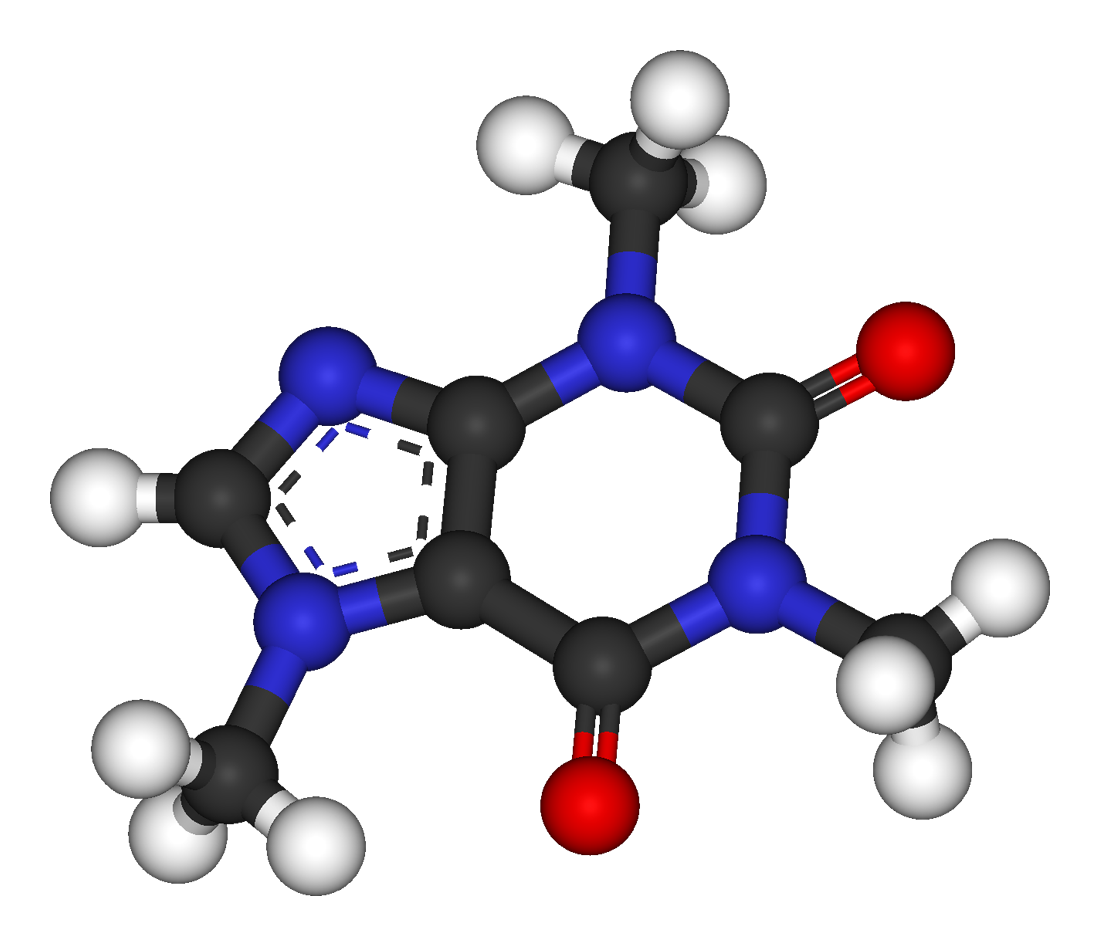
\includegraphics[scale=0.3]{molecule.png}
\end{figure}
\end{verbatim}
\end{Code}

En el caso de querer la imagen hacia la izquierda, podemos utilizar \inlinecode{\textbackslash raggedleft} en vez de \inlinecode{\textbackslash centering} Y en el caso de querer la imagen hacia la derecha, utilizamos \inlinecode{\textbackslash raggedright} Finalmente, una imagen no puede ir en un documento sin una explicaci\'on y alguna forma de referirnos a ella. Es por eso que vamos a incluir lo \'ultimo en nuestras im\'agenes:

\begin{Code}
\begin{verbatim}
\begin{figure}[h!]
\centering
\caption{Mol\'ecula de cafe\'ina en 3D.}
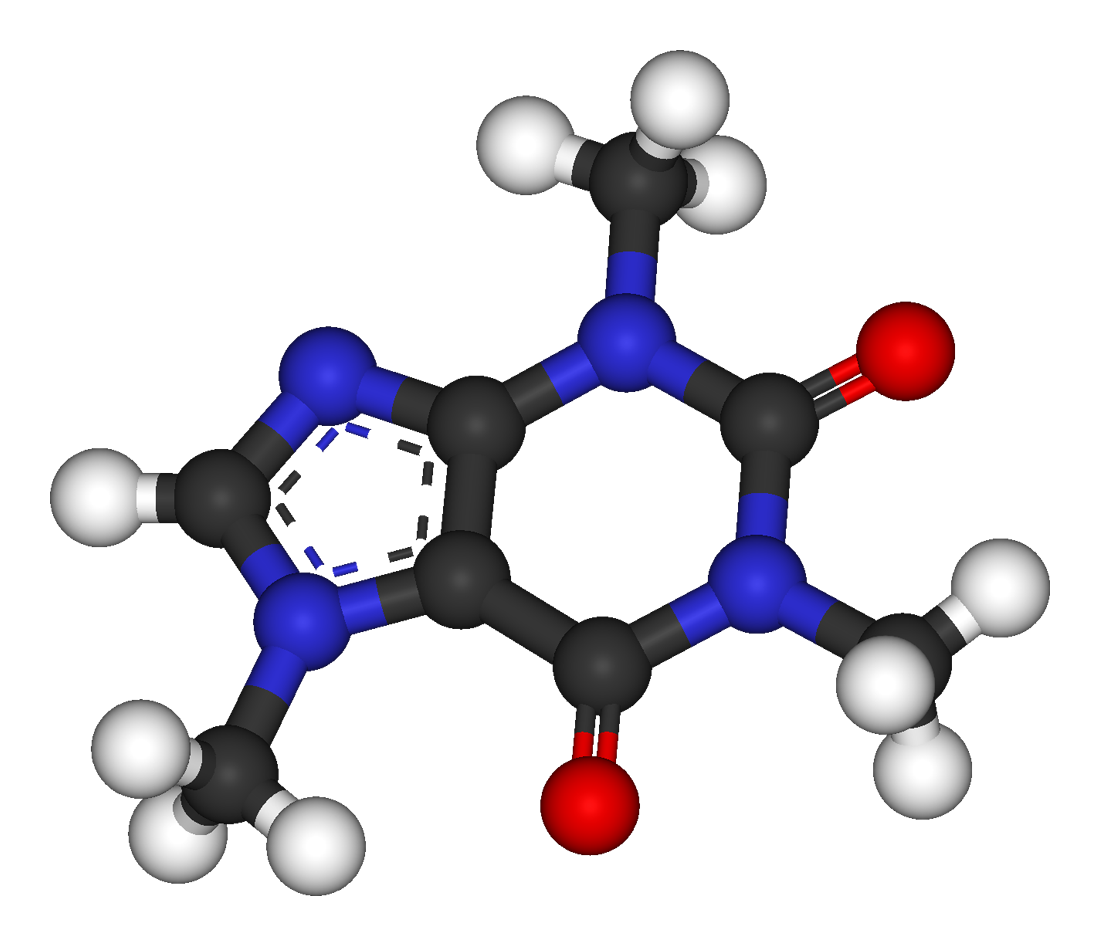
\includegraphics[scale=0.3]{molecule.png}
\label{fig:cafeina}
\end{figure}
\end{verbatim}
\end{Code}

Intentemos colocar esto en nuestro documento, observemos qu\'e pasa al construir el PDF y finalmente discutamos qu\'e es lo que creemos que hace cada parte de este conjunto. Un tip que se nos da es que \inlinecode{\textbackslash label\{fig:cafeina\}} es una forma en la que despu\'es solo tendremos que mencionar a \emph{fig:cafeina} para referirnos a esa imagen. Un ejemplo de esto lo podremos ver si inclumos \inlinecode{\textbackslash ref\{fig:cafeina\}} en alguna parte del texto en nuestro documento y lo convertimos en PDF. (Puede que a veces necesitemos de dos conversiones a PDF antes de que funcione la referencia.)\\

A decir verdad, cualquier cosa que pongamos dentro de una etiqueta \inlinecode{\textbackslash label\{\}} puede funcionar como referencia. Solemos incluir cosas como \emph{fig}, \emph{tab} o \emph{equ} para saber si se trata de una ecuaci\'on, una tabla o una figura y recordarnos mejor de lo que est\'abamos escribiendo. Y s\'i, podemos incluir una etiqueta dentro de las ecuaciones numeradas tambi\'en para poder despu\'es referirnos a ellas.\\

Otra cosa que se nos pide cada vez que hacemos un reporte o un informe es que coloquemos nuestros resultados en tablas. Esta pr\'actica hace que los resultados presentados no se vean tan desordenados, y nos permite referirnos a ellos de maneras m\'as sencillas tambi\'en. Las tablas en \LaTeX\ no suelen ser una tarea tan f\'acil al principio. Estas constan de varios ambientes uno dentro de otro y nos dejan cambiar demasiadas cosas. Algo tan sencillo como esto:

\begin{table}[h!]
\caption{Temperatura y pH del agua en las muestras del r\'io.}
\vspace*{2mm}
\centering
\begin{tabular}{c c c}
\hline
\textbf{Muestras} & \textbf{pH} & \textbf{T /$^{o}$C}\\
\hline
1 & 6.6 & 22.5\\
2 & 6.8 & 21.2\\
3 & 6.6 & 21.8\\
\hline
\end{tabular}
\label{tab:fakeresultados}
\end{table}

Se ve as\'i en c\'odigo.

\begin{Code}
\begin{verbatim}
\begin{table}[h!]
\caption{Temperatura y pH del agua en las muestras del r\'io.}
\vspace*{2mm}
\centering
\begin{tabular}{c c c}
\hline
\textbf{Muestras} & \textbf{pH} & \textbf{T /$^{o}$C}\\
\hline
1 & 6.6 & 22.5\\
2 & 6.8 & 21.2\\
3 & 6.6 & 21.8\\
\hline
\end{tabular}
\label{tab:fakeresultados}
\end{table}
\end{verbatim}
\end{Code}

Claro que hay cosas familiares, como la forma de colocar la tabla en el lugar que deseamos con \inlinecode{h!}, la manera de centrar el contenido, la manera de colocar una descripci\'on y la manera de tener una etiqueta para una referencia. Pero tambi\'en hallamos cosas nuevas como \inlinecode{\textbackslash vspace*\{2mm\}}, que deja $2mm$ entre la descripci\'on y la tabla. \inlinecode{\textbackslash hline} que coloca l\'ineas horizontales. Y, claro, el ambiente \inlinecode{tabular}\\

Este \'ultimo es el equivalente a importar las im\'agenes sin nada m\'as, como en el segmento anterior. La idea es declarar un ambiente en donde se especifique la cantidad de columnas y hacia d\'onde estar\'an orientadas al principio: \inlinecode{\{c c c\}}. Se puede utilizar \emph{c} para centrar, \emph{l} para orientar a la izquierda y \emph{r} para la derecha. Finalmente, escribimos el contenido de la tabla separando cada columna con un \inlinecode{\&} y finalizando cada fila con una dobla diagonal inversa, al igual que un p\'arrafo: \inlinecode{\textbackslash\textbackslash}\\

Como ejercicio, intentemos escribir una tabla dentro de nuestro documento, que contenga 4 columnas alineadas a la izquierda, y 5 entradas de datos. Consultemos con nuestra pareja e intentemos cambiar o agregarle algo particular nuestro.

\subsection{Art\'iculo Cient\'ifico}
Al llegar a este punto ya somos capaces de hacer la mayor parte de cosas que eramos capaces de hacer en cualquier editor de texto m\'as o menos decente. Sin embargo, hay dos cosas que debemos de notar:\\

\noindent La primera es que con \LaTeX\ podemos crear todos nuestros documentos sin tener editor de texto. Podemos escribir una tesis en el Block de Notas de Microsoft Windows que igual se va a ver profesional al convertirlo a PDF.\\

\noindent La segunda es que esto no ha terminado. \LaTeX\ es un lenguaje de estilo, y como tal, permite la creaci\'on de funciones y ambientes nuevos.\\

No vamos a ver c\'omo crear funciones o ambientes nuevos, puesto que eso es un tema para un d\'ia entero. Sin embargo, vamos a hacer uso de uno que ha sido dise\~nado para darnos mayor facilidad con algunos aspectos de \LaTeX\ y nos permitir\'a la elaboraci\'on de art\'iculos cient\'ificos en poco tiempo. En nuestra carpeta de documentos se halla uno llamado \emph{plantilla\_reporte.tex}. Abr\'amoslo y estudi\'emoslo un momento. En \'el se van a hallar las instrucciones para hacer los ejercicios de esta secci\'on. 

\subsection{Autoensablados: \'Indice y Bibliograf\'ia}
Antes de terminar, vamos a ver dos cosas muy importantes a la hora de trabajar con \LaTeX . Una es muy f\'acil, la otra no tanto. Cuando ya hemos terminado un proyecto largo y de repente revisamos en las instrucciones, a veces nos pasa que nos encontramos con las palabras de la muerte: \'indice y bibliograf\'ia. Sin embargo, gracias a lo que ya tenemos hecho en nuestros documentos, agregar el \'indice en \LaTeX\ es algo s\'uper-simple. Vamos antes de la car\'atula o en la primera p\'agina y colocamos la siguiente secuencia: \inlinecode{\textbackslash tableofcontents} Con esto ya tenemos el \'indice. Si deseamos que este no se mezcle con el resto de nuestro contenido y tenga una p\'agina dedicada, despu\'es de \'el agregamos otra secuencia: \inlinecode{\textbackslash newpage} Y eso es todo.\\

En el caso de la bibliograf\'ia si se trata de algo m\'as elaborado. Existen varios paquetes para autoensamblar bibliograf\'ias basadas en documentos de texto con la informaci\'on necesaria. Bib\TeX\ es un caso, pero la mayor\'ia de proyectos no han \emph{madurado} lo suficiente como para poderlos llamar est\'andar. En ese caso, vamos a trabajar con una forma de bibliograf\'ia muy sencilla que generalmente se incluye dentro de un documento \LaTeX\ inmediatamente.\\

Un detalle que debemos considerar antes de comenzar a llenar nuestro documento con bibliograf\'ias y citas es que estas pueden tener un estilo particular dado por un paquete. En nuestro caso vamos a incluir un paquete de estilos y vamos a configurar un tipo de citas. Nos toca colocar las siguientes l\'ineas al principio de nuestro documento para cumplir con la consistencia del paquete a utilizar:

\begin{Code}
\begin{verbatim}
\usepackage{natbib}
\bibliographystyle{apa}
\end{verbatim}
\end{Code}


Ahora vamos a trabajar con nuestro \'ultimo ambiente: \inlinecode{thebibliography} y adem\'as de eso, vamos a crear nuestra primera entrada bibliogr\'afica. Para ello vamos a escoger un libro que seguro todos hemos utilizado antes \citep{bib:mcmurry}. Por ello, nuestro c\'odigo se ver\'a de la siguiente manera:

\begin{Code}
\begin{verbatim}
\begin{thebibliography}{99}

\bibitem[McMurry, 1992]{bib:mcmurry}
    John McMurry.
    (1992).
    \emph{Organic Chemistry}.
    (3rd ed).
    Pacific Grove, California:
    Brooks/Cole Publishing Company.

\end{thebibliography}
\end{verbatim}
\end{Code}

Esto tiene mucha informaci\'on, pero vamos paso a paso. Lo primero extra\~no que notamos es que al crear el ambiente, tambi\'en incluimos \inlinecode{\{99\}} Esto es para dar un m\'aximo de cu\'antas bibliograf\'ias se incluir\'an. De no incluirse esto, \LaTeX\ dar\'a error indicando que algo falta. Lo siguiente que notamos es la secuencia \inlinecode{\textbackslash bibitem[]\{\}} Esta inicia una nueva entrada en la bibliograf\'ia. Entre los corchetes va la manera en la que se desea mostrar la cita, y entre las llaves la etiqueta con la que haremos referencia a esa cita. Lo dem\'as es solo la informaci\'on del libro a manera de leerse m\'as f\'acil; podr\'iamos colocarla en una sola l\'inea.\\

Si ponemos atenci\'on, la bibliograf\'ia es como un ambiente numerado. Las diferencias son que hay que colocar un m\'aximo de entradas, y que cada entrada debe llevar su forma de representar la cita y su etiqueta para citarse. Tomando esto \'ultimo en cuenta, no hemos visto c\'omo citar algo de la bibliograf\'ia. Para ello se utiliza \inlinecode{\textbackslash citep\{\}} En nuestro caso en particular, tendr\'iamos que hacerlo de la siguiente manera: \inlinecode{\textbackslash citep\{bib:mcmurry\}} Con eso ya podemos colocar la cita donde nos plazca. Claro, es preferible incluirla al final de un p\'arrafo. Ahora, para ver c\'omo se ve el resultado de nuestro c\'odigo, podemos analizar la cita que incluimos hace 2 p\'arrafos y las \textbf{Referencias} que se presentan a continuaci\'on\footnote{La palabra \textbf{Referencias} no es una secci\'on que se haya definido en el documento. Esto lo incluye \LaTeX\ como parte de la bibliograf\'ia.}.

\begin{thebibliography}{99}

\bibitem[McMurry, 1992]{bib:mcmurry}
    McMurry, John.
    (1992).
    \emph{Organic Chemistry}.
    (3rd ed).
    Pacific Grove, California:
    Brooks/Cole Publishing Company.

\end{thebibliography}
\newpage
\subsection{Tesis}
Por el momento no existe en muchas partes, pero ser\'ia muy interesante que as\'i como existe un formato para reporte cient\'ifico, existiera el formato de tesis en \LaTeX\ para que solo tuvieramos que llenar. Ser\'ia particular de la facultad a la que pertenecemos y solo necesitar\'iamos de escribir la informaci\'on necesaria sin tener que estar pensando en el formato, la numeraci\'on de las p\'aginas, las figuras, las gr\'aficas, etc. Todo esto se podr\'ia automatizar llegando a un documento de texto y una o dos hojas de estilo. Este es un proyecto que podr\'ia hacerse como ejercicio avanzado para quien desee aventurarse.

\subsection{Comentarios Finales}
Muchas felicidades, has completado el cuarto d\'ia del taller de QCA. Tu conocimiento ya te permite escribir reportes e informes de una manera m\'as profesional y aceptada por la comunidad cient\'ifica. \LaTeX\ es un tema del que se han escrito hasta libros (utilizando el mismo \LaTeX ); es muy vasto y con muchas posibilidades.\\

Si deseas profundizar m\'as en el uso de \LaTeX , ser\'ia recomendable que comenzaras otra vez desde el principio viendo en qu\'e var\'ian exactamente los diferentes tipos de documento. Luego pasar a ver casos especiales como rotaci\'on de una sola p\'agina, c\'omo utilizar colores en el texto, c\'omo incluir espacios en blanco, c\'omo trabajar con varias columnas, notas al pie, notas al margen, matrices, hiperv\'inculos, gr\'aficas autogeneradas, estructuras qu\'imicas autogeneradas, c\'omo lograr que algo se autonumere, etc. hasta terminar con programaci\'on y dise\~no de clases de documento o p\'aginas de estilo. Finalmente, ser\'ia recomendable que revisaras c\'omo se trabaja con \LaTeX\ para \emph{realmente} publicar en revistas cient\'ificas. Para eso, puedes revisar algunas editoriales como \href{http://pubs.acs.org/page/4authors/submission/tex.html}{ACS}, \href{http://www.rsc.org/Publishing/Journals/guidelines/AuthorGuidelines/AuthoringTools/Templates/tex.asp}{RSC}, \href{http://www.elsevier.com/authors/author-schemas/latex-instructions}{Elsevier} y \href{https://www.springer.com/gp/authors-editors/book-authors-editors/manuscript-preparation/5636}{Springer} por mencionar algunas. Puedes llegar a hacer todo lo que te imaginas con esto.\\

Felicidades nuevamente, ma\~nana terminamos con la primera semana viendo la introducci\'on a programaci\'on con Python. \'Animo, lo mejor est\'a por venir!

\section*{Licencia}

\noindent 
\includegraphics{img/cc_big.png}

\noindent Taller de Qu\'imica Computacional Aplicada by \href{http://github.com/zronyj/TQCA}{Rony J. Letona} is licensed under a \href{http://creativecommons.org/licenses/by-sa/4.0/}{Creative Commons Attribution-ShareAlike 4.0 International License}.

\end{document}
